\documentclass{article}\usepackage[]{graphicx}\usepackage[]{color}
%% maxwidth is the original width if it is less than linewidth
%% otherwise use linewidth (to make sure the graphics do not exceed the margin)
\makeatletter
\def\maxwidth{ %
  \ifdim\Gin@nat@width>\linewidth
    \linewidth
  \else
    \Gin@nat@width
  \fi
}
\makeatother

\definecolor{fgcolor}{rgb}{0.345, 0.345, 0.345}
\newcommand{\hlnum}[1]{\textcolor[rgb]{0.686,0.059,0.569}{#1}}%
\newcommand{\hlstr}[1]{\textcolor[rgb]{0.192,0.494,0.8}{#1}}%
\newcommand{\hlcom}[1]{\textcolor[rgb]{0.678,0.584,0.686}{\textit{#1}}}%
\newcommand{\hlopt}[1]{\textcolor[rgb]{0,0,0}{#1}}%
\newcommand{\hlstd}[1]{\textcolor[rgb]{0.345,0.345,0.345}{#1}}%
\newcommand{\hlkwa}[1]{\textcolor[rgb]{0.161,0.373,0.58}{\textbf{#1}}}%
\newcommand{\hlkwb}[1]{\textcolor[rgb]{0.69,0.353,0.396}{#1}}%
\newcommand{\hlkwc}[1]{\textcolor[rgb]{0.333,0.667,0.333}{#1}}%
\newcommand{\hlkwd}[1]{\textcolor[rgb]{0.737,0.353,0.396}{\textbf{#1}}}%
\let\hlipl\hlkwb

\usepackage{framed}
\makeatletter
\newenvironment{kframe}{%
 \def\at@end@of@kframe{}%
 \ifinner\ifhmode%
  \def\at@end@of@kframe{\end{minipage}}%
  \begin{minipage}{\columnwidth}%
 \fi\fi%
 \def\FrameCommand##1{\hskip\@totalleftmargin \hskip-\fboxsep
 \colorbox{shadecolor}{##1}\hskip-\fboxsep
     % There is no \\@totalrightmargin, so:
     \hskip-\linewidth \hskip-\@totalleftmargin \hskip\columnwidth}%
 \MakeFramed {\advance\hsize-\width
   \@totalleftmargin\z@ \linewidth\hsize
   \@setminipage}}%
 {\par\unskip\endMakeFramed%
 \at@end@of@kframe}
\makeatother

\definecolor{shadecolor}{rgb}{.97, .97, .97}
\definecolor{messagecolor}{rgb}{0, 0, 0}
\definecolor{warningcolor}{rgb}{1, 0, 1}
\definecolor{errorcolor}{rgb}{1, 0, 0}
\newenvironment{knitrout}{}{} % an empty environment to be redefined in TeX

\usepackage{alltt}
\usepackage{Sweave}
\usepackage{graphicx}
\usepackage{tabularx}
\usepackage{amsmath}
\usepackage[small]{caption}
\usepackage{gensymb}
\usepackage{float}
\setkeys{Gin}{width=0.8\textwidth}
\setlength{\captionmargin}{30pt}
\setlength{\abovecaptionskip}{0pt}
\setlength{\belowcaptionskip}{10pt}
\topmargin -1.5cm        
\oddsidemargin -0.04cm   
\evensidemargin -0.04cm
\textwidth 16.59cm
\textheight 21.94cm 
\pagestyle{empty}
\parskip 7.2pt
\renewcommand{\baselinestretch}{1.5}
\parindent 0pt

%% R Script


%% Making a Bibliography
\usepackage[backend=biber, bibencoding=ascii, style=nature]{biblatex}
\bibliography{library.bib}
\IfFileExists{upquote.sty}{\usepackage{upquote}}{}
\begin{document}
\SweaveOpts{concordance=TRUE}
\title{Comparing Methodologies for Calculating False Spring Index}
\author{C Chamberlain}
\date{\today}
\maketitle 

\renewcommand{\thetable}{\arabic{table}}
\renewcommand{\thefigure}{\arabic{figure}}
\renewcommand{\labelitemi}{$-$}
%%%%%%%%%%%%%%%%%%%%%%%%%%%%%%%%%%%%%%%%%%%%%%%
\section*{Introduction}

Plants that grow in temperate environments are at risk of being exposed to late spring freezes, which can be detrimental to plant growth. According to Gu et al. (2008), there are two phases involved in late spring freezing: rapid vegetative growth prior to the freeze and the post freeze setback. This combined process is known as a false spring. Freeze and thaw fluctuations can cause xylem embolism and decreased xylem conductivity which can result in crown dieback \cite{Gu2008}. More frequently, however, plants that have been exposed to a false spring will experience leaf loss and slower canopy development \cite{Hufkens2012}. With anthropogenic climate change, the severity of damage incurred from a false spring phenomena is predicted to be heightened due to earlier spring onset and greater fluctuations in temperatures. It is anticipated that there will be a decrease in false spring occurrence overall but the severity of temperature variation is likely to increase \cite{Allstadt2015}. 

Different species exhibit varying responses to late spring freezing events and the level of damage also varies across phenophases. Generally, reproductive phases are more sensitive to false spring events than vegetative phases and developing leaves are more susceptible to damage than opening buds or expanding shoots \cite{Peterson2014}. False spring events also put seedling and sapling trees at greater risk to damage than adult trees \cite{Vitasse2014}. Warm temperatures earlier in the year (i.e. in February) do not seem to affect species, most likely because it is too soon for bud burst to take place and sufficient chilling has not yet occurred. Frost damage usually occurs when there is a warmer than average March, a freezing April, and enough growing days between the high temperatures and the last freeze date {Augspurger2013}. In a study performed by Peterson and Abatzoglou (2014), it had been determined that 7 days between bud burst and last freeze date is a significant parameter. There is much debate over the definition of freezing temperatures and has resulted in two types of freezes: a "hard" freeze at -2.2$^{\circ}$C and a "soft" freeze at -1.7$^{\circ}$C \cite{Augspurger2013, Kodra2011, Vavrus2006}.

\section*{Rethinking False Spring}

\section*{Methods}

In this study, we aim to establish an index, known as a False Spring Index (FSI), that signifies the likelihood of a damage to occur from a late spring freeze on forest plant species at Harvard Forest, Petersham, Massachusetts (42$^{\circ}$31'54.2"N 72$^{\circ}$11'23.8"W). FSI evaluates day of bud burst, number of growing degree days, and day of last spring freeze through a simple equation as seen below \cite{Marino2011}. A "soft" freeze parameter is chosen for this study. By integrating a more strict parameter with a higher freezing temperature, we will be able to establish a greater evaluation of level of risk. 

\[ FSI = Julian Date (Last Spring Freeze) - Julian Date (Bud Burst) \]

If FSI is a positive number and greater than 7, then crown dieback is more likely to occur. The date of last spring freeze was gathered from the Fisher Meteorological Station which was downloaded from the Harvard Forest web page (data available online\footnote{http://harvardforest.fas.harvard.edu/meteorological-hydrological-stations}). The Tmin values were used and the Last Spring Freeze was  determined from the latest Julian date that the temperature reached -1.7$^{\circ}$C or below. The date of bud burst was evaluated through three different methodologies. The first method for collecting bud burst was from observational data recorded for 33 tree species by Dr. John O'Keefe at Harvard Forest from 1990 to present \cite{OKeefe2014}. Dr. O'Keefe defines bud burst as 50\% leaf emergence. The second data set was provided from PhenoCam data, which are field cameras, placed in Harvard Forest, take real-time images of plant growth and are programmed to record initial green up. The final set was collected through the USA National Phenology Network (USA-NPN), using their Data Visualization tool to gather Extended Spring Index values (SI-x). The SI-x value is the time of leaf out as monitored from historical dates of bud burst using honeysuckle and lilac clones around the U.S. and combining that information with daily recordings from local weather stations \cite{USA-NPN2016, Ault2015, Ault2015a, Schwartz2013, Schwartz1997}. Through assessing past years' weather and bud burst, scientists are able to determine general weather trends that subsequently lead to leaf out. Based on these trends, SI-x values can be calculated from daily weather data \cite{USA-NPN2016}. %%%Lizzie, I am only assessing Harvard Forest data here to compare the three methods and also there is only one date of bud burst that we can use for SH at this time. I should be able to calculate a second FSI value for SH once Eric is home from vacation and I can get the weather data for 2015. At that time, I'll integrate the SH information!%%%
\newline
PhenoCam data is not available for Harvard Forest until 2008 and observation data is only recorded through 2014, so this evaluation assesses FSI values from 2008 through 2014. 
\section*{Results}
Date of bud burst varied between the three methodologies used. For the observational data, date of bud burst was determined by finding the mean date for all species observed in the study performed by Dr. O'Keefe (2014). %%%Lizzie, should I use first date of bud burst instead? I can change this method to determine observed bud burst date.%%% 
As is seen in Table 1, Observed Bud Burst dates and PhenoCam Bud Burst dates are similar, whereas SI-x dates gathered from the USA-NPN are recorded as much earlier in the year.

% latex table generated in R 3.3.1 by xtable 1.8-2 package
% Mon Nov 14 08:13:05 2016
\begin{table}[ht]
\centering
\caption{Last Freeze julian dates recorded from 2008 to 2014 and day of bud burst recorded for all three methodologies.} 
\begin{tabular}{rrrrr}
  \hline
 & year & Last Freeze & SI-x & Observed \\ 
  \hline
1 & 2008 & 122 & 113 & 119.62 \\ 
  2 & 2009 & 103 & 113 & 118.12 \\ 
  3 & 2010 &  87 &  97 & 105.62 \\ 
  4 & 2011 & 112 & 113 & 123.75 \\ 
  5 & 2012 & 120 &  85 & 110.38 \\ 
  6 & 2013 & 112 & 113 & 122.50 \\ 
  7 & 2014 & 110 & 113 & 130.00 \\ 
   \hline
\end{tabular}
\end{table}

The FSI values were calculated for each methodology from 2008 to 2014 using the formula based of the study performed by Marino et al. (2011). Table 2 shows that the Observed and PhenoCam FSI values are all negative from 2008 through 2014. The FSI values from the NPN are, on average, much higher in comparison to the other two methods. In 2008 and 2012, FSI is higher than the significant parameter given of 7, indicating a possibly damaging false spring event. 
\begin{table}[ht]
\centering
\caption{False Spring Indices calculated using all three methodologies} 
\begin{tabular}{rrrrrr}
  \hline
 & year & FSI\_npn & FSI\_sm & FSI\_obs & FSI\_cam \\ 
  \hline
1 & 2008 &   9 & 2.38 & -1.88 &  -3 \\ 
  2 & 2009 & -10 & -15.12 & -17.53 & -17 \\ 
  3 & 2010 & -10 & -18.62 & -24.24 & -24 \\ 
  4 & 2011 &  -1 & -11.75 & -14.59 & -11 \\ 
  5 & 2012 &  13 & 9.62 & -18.24 & -20 \\ 
  6 & 2013 &  -2 & -10.50 & -13.59 & -10 \\ 
  7 & 2014 &  -5 & -20.00 & -24.53 & -21 \\ 
   \hline
\end{tabular}
\end{table}


A graphical representation of the FSI values compared across the three methodologies can be seen in Figure 1.  Again, it is evident that the FSI values determined from the USA-NPN bud burst dates are much higher.

\begin{figure}
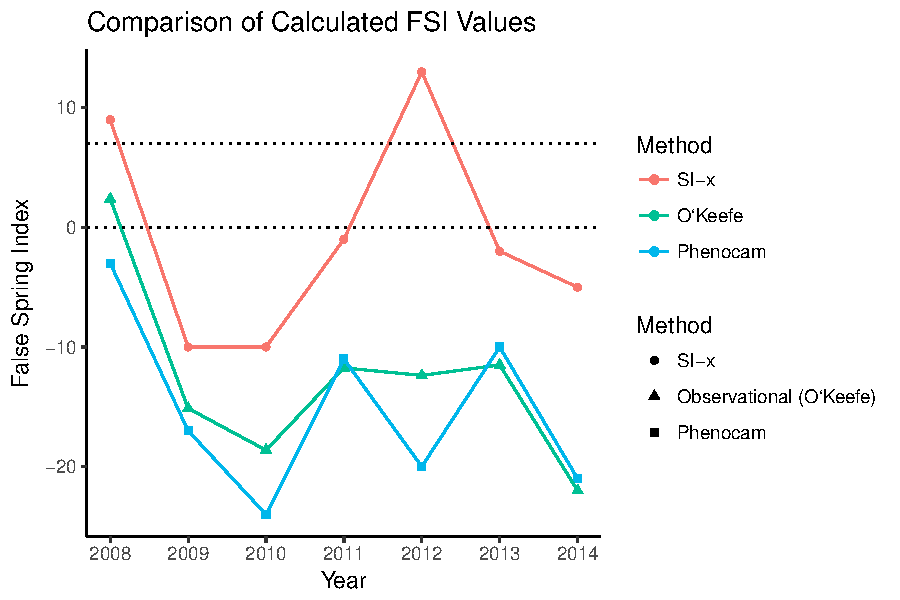
\includegraphics[width=\maxwidth]{figure/fsifig-1} \caption[A scatterplot indicating FSI values from 2008 to 2014 for each methdology used in this study]{A scatterplot indicating FSI values from 2008 to 2014 for each methdology used in this study. PhenoCam FSI values are red, Observed FSI values are blue, and USA-NPN FSI values are green.}\label{fig:fsifig}
\end{figure}



A Pearson Correlation was used to determine the strength of association between the three methods used in the study. As indicated in Table 3, the FSI values from Observed data and PhenoCam data are strongly correlated (r=0.9533164), whereas the FSI values calculated using the USA-NPN data is not strongly correlated to either the Observed FSI values (r=0.5604386) or the PhenoCam FSI values (r=0.4242059).

\begin{table}[ht]
\centering
\caption{Pearson Correlation Coefficients shown comparing the strength of association between the FSI values calculated across all three methodologies.} 
\begin{tabular}{rrrrrr}
  \hline
 & year & FSI\_npn & FSI\_sm & FSI\_obs & FSI\_cam \\ 
  \hline
year & 1.00 & -0.03 & -0.21 & -0.54 & -0.37 \\ 
  FSI\_npn & -0.03 & 1.00 & 0.95 & 0.56 & 0.42 \\ 
  FSI\_sm & -0.21 & 0.95 & 1.00 & 0.57 & 0.38 \\ 
  FSI\_obs & -0.54 & 0.56 & 0.57 & 1.00 & 0.95 \\ 
  FSI\_cam & -0.37 & 0.42 & 0.38 & 0.95 & 1.00 \\ 
   \hline
\end{tabular}
\end{table}


%Figure 2 shows the FSI values for the PhenoCam data and the Observed data. As seen in the scatter %plot, values are very similar.

%<<label=hf, results="asis", message=FALSE, echo=FALSE, fig.pos="H", fig.cap="A scatterplot indicating FSI values from 2008 to 2014 for PhenoCam and Observed data. PhenoCam FSI values are red and Observed FSI values are blue.", fig.align='center'>>=
%plot(hf)
%@

%<<label=gradient, results="asis", message=FALSE, echo=FALSE, fig.cap="A scatterplot comparing FSI values for Harvard Forest and Saint Hippolyte from 2014 to 2015", fig.align="center">>=
%plot(gradient)
%@

\section*{Conclusions}
Our projections indicate that observational FSI values are highly comparable to PhenoCam FSI values, rendering both justifiable methods for determining potential risk involved in late spring freezes. Even though bud burst is defined differently between Dr. O'Keefe and the PhenoCam observations, the dates of bud burst are very similar. The SI-x dates gathered from the USA-NPN are significantly different from the other two methods, which is likely due to fact that the USA-NPN is assessing bud burst for honeysuckle and lilacs rather than forest tree species. Through the use of PhenoCam data, researchers could gather dates of bud burst across multiple locations at once, making it a more effective method than observational data. 

%\newpage
%\printbibliography

\end{document}
